\chapter{含风电电力系统的脆弱性研究}
\label{cha:theory}

\section{引言}
\label{sec:index3}
近年来在电力系统的研究领域中,脆弱性一直是个热点的研究课题。许多学者认为系统脆弱性是一种隐形性能,在正常工作时并不显见。一旦外界对系统产生了特定的影响,那么系统的性能参数就会迅速变坏,甚至不能稳定工作。对于含风电的电力系统本身对环境有着较大的依赖性,而其电能质量的输出仍要满足要求,具有脆弱性的系统导致的后果将十分严重。因此,分析含风电电力系统的脆弱性很有必要。

针对含风电电力系统,本章通过分析系统脆弱性存在的原因得出系统的脆弱性本质以及其数学描述,进而得出一个较为清晰的系统脆弱性概念。根据脆弱性的定义,分别从系统的结构和系统的状态两个角度对脆弱性进行分析研究。结构脆弱性从系统拓扑的角度,研究了系统在运行中,保持其拓扑完整性的能力。而状态脆弱性则专注研究外界环境的变化使系统暴露出的缺陷,即向坏的方向发展的趋势。

\section{含风电电力系统脆弱性}
\label{sec:defina}
对于含风电的电力系统而言,外界环境瞬态多变,在这种情况下,系统会不会暴露出自身的缺点,是该系统的性能分析中重要的一部分。针对系统自身存在的在一定条件下才会暴露的缺陷,本节做了较为深入的探讨。
\subsection{含风电电力系统脆弱性本质}
\label{sec:network}
脆弱性本身是系统的一个隐形特征,在正常工作情况下不会显现。只有针对特定的工作情况或者受到特定的干扰时,系统性能参数才会快速变差,表现出脆弱性的特征。风力发电系统本身就依靠外界风力,对环境的依赖性较强。含风电的电力系统在运行期间,产生的电能的质量除了取决于自身的可靠性和固有能力,组成系统的抗干扰能力也是影响其正常工作的关键因素。

随着风电渗透密度的增大,负荷需求时变性的增大,对系统的考验越来越大。而系统内部拓扑的设计、各母线节点的连接情况,风电功率的特性都将影响着系统的运行状态。如下图,需要在脆弱源、脆弱环节、系统性能之间建立关系,根据性能特点和实际情况来进行脆弱性分析。
\begin{figure}[H] % use float package if you want it here
  \centering
  \includegraphics[height=7.3cm]{vulnerability_exist.pdf}
  \caption{脆弱性存在的原因}
  \label{fig:vulnerability_exist}
\end{figure}

对系统的脆弱性分析,主要包括两个环节:

$(1)$通过分析“脆弱源$\longrightarrow$脆弱环节”的关系来判断系统中易受脆弱源影响的节点。

$(2)$通过分析“脆弱环节$\longrightarrow$系统性能”的关系来评估受干扰的脆弱环节对系统性能的影响程度,又可称为脆弱程度。

\subsection{含风电电力系统脆弱性数学描述}
\label{sec:network}
特别地,对于含风电电力系统,系统的性能变化的主要原因是风力发电系统参数的变化和外界扰动信号,参数的变化和外界的干扰信号可以看做一个事件对系统发动的“攻击”,这个“攻击”导致系统性能指标下降,那就是脆弱性的表现。

设系统$S$的某性能指标$E$,如果存在事件$I$,当它对系统的某个或者某些参数产生影响,使得系统性能指标变化,即
\begin{equation}
\label{equ:chap3:Index0}
E(I^{+})-E(I^{-})\neq 0
\end{equation}
则称系统$S$具有脆弱性,$I^{+}$为脆弱事件发生前,$I^{-}$为脆弱事件发生后,导致系统性能改变的根本因素称为脆弱源。

综合上述对含风电电力系统脆弱性本质的研究以及数学描述的探究,本文对含风电电力系统的脆弱性做如下定义:

当系统由于工作环境导致自身部分参数发生改变时,系统承受不确定性的能力迅速变差,这种不易暴露的系统自身的缺陷即为脆弱性。

\section{含风电电力系统结构脆弱性研究}
\label{sec:powersys}
风力发电系统的结构主要指的是除发电机、负荷之外,电能被输送的网络的拓扑。拓扑是整个网络性能的基础,它决定了电能是否能够被安全、有效、可靠的输送到负荷端。但是,受外界环境的干扰、人为干预、不可抗力的影响,拓扑的结构并非一成不变,其组成元素都有遭到破坏的可能。因此,有必要衡量拓扑的各个组成元素在结构上的重要性,这对于提前加强防范、预先保护有着重要的意义。

本文在前人研究的基础上对结构脆弱性提出了新的定义:电力系统的结构脆弱性是指电力系统自身组成因素保持其结构完整的能力。对系统结构完整性贡献的程度越高、对拓扑完整性的影响程度越高的组成元素被称为系统结构的脆弱点。因此,对电力系统的结构越重要,影响越关键的组成因素的脆弱性越高。

风力发电系统的结构建模有多种,本文分别从复杂网络的角度和互联网网页重要度排序的角度进行研究。前者将电网抽象为一个加权无向图,后者将电网等效为一个有向图。二者出发的角度不同,建模方式不同,但是都从结构上对电网节点的重要性进行了评估。本文对这两种建模方法进行了研究和对比,将各自的模型指标在第四章中进行了融合评估。

\subsection{基于复杂网络的结构脆弱性研究}
\label{sec:network}
复杂网络的基本思想是将一个复杂系统抽象为网络,其中系统中的单个个体被视为网络的节点,而个体之间的联系被视为网络的边,由此建立复杂网络模型。对于含风电电力系统而言,系统中的母线可以被视为节点,而母线之间的电气连接可以被视为边,线路上的阻抗为权重,因此整个系统可以被等效为一个加权无向图\cite{networkE2,networkE3,networkE4}。

复杂网络理论中描述网络的特征参数有特征路径长度、节点度和节点度累计分布、聚类系数、介数和介数分布等\cite{networkE}。其中,度是复杂网络中的一个基本且常用的参数,其公式化的定义如下:
\begin{equation}
\label{equ:chap3:Index01}
k_i=\sum_{j=1,j\neq i}^{N}a_{ij}
\end{equation}

其中,$a_{ij}$为复杂网络邻接矩阵的元素,为$0$代表$i,j$不相连,为$1$代表$i,j$相连。

对于有权网络,节点度的概念扩展为节点的连接强度,公式定义如下:
\begin{equation}
\label{equ:chap3:Index02}
s_i=\sum_{j=1,j\neq i}^{N}w_{ij}
\end{equation}

其中,$w_{ij}$为节点$i,j$之间的连接强度。

两种定义只考虑单方面的度的定义太过片面,第一种侧重于节点的连接数量,适合无权网络;第二种则考虑节点的连接强度,适合有权网络。因此,本文综合考虑节点连接数量与连接强度,结合电力网络的特点,定义“电气度”概念如下:
\begin{equation}
\label{equ:chap3:Index03}
e_i=\sum_{j=1,j\neq i}^{N}ea_{ij}\cdot ew_{ij}
\end{equation}
其中,$ea_{ij}$为网络中邻接节点的连接情况,为$0$代表$i,j$不相连,为$1$代表$i,j$相连。而$ew_{ij}$代表支路潮流上的视在功率的大小。电气度衡量了节点在拓扑形成与结构中承担的应力大小,是网络中衡量节点重要性的重要参数。

介数作为复杂网络的关键参数之一,被用来描述节点或者边在信息、能量传递中的重要程度。介数的概念在电力系统被称为电气介数,它反映了网络节点、支路在整个电能输送过程中的贡献程度\cite{elecDu1,elecDu2,elecDu3}。

假设一个电网具有$a$个母线节点,$b$条电气连接的边,那么支路$l_{mn}$的电气介数计算公式如下:
\begin{equation}
\label{equ:chap3:Index1}
C_{B}(m,n)=\left|\sum_{i\in\mathbf{G},j\in\mathbf{D}}w_{ij}P_{mn}(i,j)\right|
\end{equation}

其中,$G$,$D$分别为发电节点、负荷节点的集合。$P_{mn}(i,j)$是单位有功功率注向发电节点$i$和负荷节点$j$时,支路$l_{mn}$上产生的有功功率。$w_{ij}$是发电节点$i$和负荷节点$j$的节点对间传输电能的权重值,大小为$min(|P_i|,|P_j|)$,分别代表了发电节点$i$在发电节点功率总和的比率和负荷节点$j$在负荷节点功率总和的比率。

电网中节点的分类分为发电节点,负荷节点,中间节点。所有的功率都是从发电节点向负荷节点传输,因此需要对上述公式进行修正得到如下的节点电气介数计算公式。式~(\ref{equ:chap3:Index2})中,$F(k)$指的是与节点$k$相连的所有边的集合,$C_B(k,l)$为对应支路的电气介数。节点的电气介数与拓扑中所连支路的电气介数有直接关系。
\begin{equation}\label{equ:chap3:Index2}
C_B(k)= \begin{cases}
        \displaystyle\frac{1}{2}\left(\sum\limits_{l\in\mathbf{F(k)}}{C_B(k,l)}+\sum\limits_{i\in\mathbf{D}}{w_{ki}}\right), &  k\in\mathbf{G} \\
        \displaystyle\frac{1}{2}\left(\sum\limits_{l\in\mathbf{F(k)}}{C_B(k,l)}+\sum\limits_{i\in\mathbf{G}}{w_{ik}}\right), &  k\in\mathbf{D} \\
        \displaystyle\frac{1}{2}\left(\sum\limits_{l\in\mathbf{F(k)}}{C_B(k,l)}\right) & k\not\in\mathbf{G},k\not\in\mathbf{D} \\
      \end{cases}
\end{equation}

由此,所有节点的电气介数计算流程如图\ref{fig:nodeBetweenPro}。
\begin{figure}[H] % use float package if you want it here
  \centering
  \includegraphics[height=12.7cm]{nodeBetweenProcess.pdf}
  \caption{电气介数计算流程}
  \label{fig:nodeBetweenPro}
\end{figure}

从流程图可以看出,节点的电气介数综和考虑了所连支路对其的影响。而支路的电气介数则衡量了所有发电-负荷节点对支路潮流的影响,从而在分析时,不仅考虑了拓扑的影响而且增加了能量变化的考虑,使得结构的衡量更完善。电气介数不局限于能量、信息沿着网络的最短路径传播,更体现了电能在整个网络支路的分布情况。同时,电气介数还分别考虑了发电节点和负荷节点的变化影响,改变他们的容量,网络各节点的重要性也会发生变化,因此,电气介数更符合实际电网的变化情况。

\subsection{基于$PageRank$的结构脆弱性研究}
\label{sec:pagerank}
$PageRank$最早是被用来作为互联网网页结构的模型,并且对所有网页的重要度进行量化评估的一种算法\cite{PR1,PR2,PR3}。在众多计算互联网网页的相关性的算法中,$PageRank$是名气最大,且最早被谷歌浏览器采用的。$PageRank$的基本思想是一个网页的重要性依赖于所有链接向它的其他网页。比如,网页$i$有链接指向网页$j$,如果有很多其他网页有链接指向网页$j$,那么我们认为,网页$j$是非常重要的。另一方面,若只有一个网页有链接指向网页$j$,但是这个网页是一个权威性很高的网址,如谷歌,百度等网页,我们认为网页$j$也非常重要,因为由受欢迎、权威的网页指向它,这份重要性将会传递下来。

电网中,每条支路上的潮流是有确定的方向的,所以可以被视为一个有向图。其中,每个母线节点被视为一个网页,母线节点之间的电气连接被视为网页中的超链接,根据电流的方向决定超链接的方向。互联网与电网的$PageRank$的拓扑模型比较如表~\ref{tab:PRComparision}。已有的研究中,大多学者在$PageRank$模型的网页出链的处理上采用均分的思想\cite{PRNET},本文在综合考虑潮流能量对结构的影响下,认为出链是按照实际的潮流的比重进行分配的。

即按照网页的超链接可以传递重要性的思想,假设$A$节点拥有~3~个出链,它会分别按照视在功率的比例分别传递给所指向的$B$、$C$、$D$三个节点,按照能量的分布作为权重。根据重要性传递规则,可以得到能量转移矩阵$A$。对于没有出链的节点,则按照$PageRank$的算法,认为该节点对所有节点都出链,从而解决终止点的问题。因为电网的潮流能量分布中不存在自己指向自己的连接,故不存在陷阱问题,因此不予考虑。
\begin{table}[htb]
  \centering
  \caption{互联网与电网的$PageRank$拓扑模型比较}
  \label{tab:PRComparision}
    \begin{tabular}{C{4.5cm}C{4.5cm}C{4cm}}
      \toprule
      互联网 & 电网 & $PageRank$拓扑 \\
      \midrule
      网页 & 母线 & 节点\\
      超链接 & 输电支路 & 有向边\\
      指向该网页的网页数目 & 母线进线数目 & 入度\\
      该网页指向的网页数目 & 母线出线数目 & 出度\\
      \bottomrule
    \end{tabular}
\end{table}

$PageRank$算法应用于电网拓扑的具体步骤为:

$(1)$假定初始服从均匀分布,即每个母线节点的重要性都是相同的,即对于一个一共有$n$个节点的系统而言,赋予每个网页初始相同的$PR$值,一般都为1。

$(2)$根据电网的实际潮流计算每条连接上的视在功率得到能量分布权重的矩阵P,再根据公式\ref{equ:chap3:Index3}得到能量转移矩阵A。

$(3)$迭代计算,由于每个超链接的存在都会增加对应网页的$PR$值,所以通过考虑潮流连接、能量转移情况对各个母线节点的$PR$值进行迭代更新。

$(4)$最后,经过若干次的迭代后,各个母线节点的$PR$值会趋于一个稳定的值。
\begin{equation}
\label{equ:chap3:Index3}
PR(p_i)=\frac{1-q}{N}+q\sum\limits_{p_j\in\mathbf{M_{p_i}}}{\frac{PR(p_j)}{L(p_j)}}
\end{equation}

式~(\ref{equ:chap3:Index3})中,$p_i$是被计算的节点,$M_{p_i}$是节点$p_i$的入链节点集合,$L(p_j)$是节点$p_j$的出链数目,$N$是节点总数目。$q$为阻尼系数,一般取~0.85~,引入该参数是为了解决出链为零的节点在模型计算中带来的问题,代表了当前的母线节点没有遭到破坏正常运行的概率。$1-q$则代表了节点遭到意外破坏退出运行的概率。从公式中可以看出,$p_i$节点的$PR$值与和它相连的$p_j$节点的$PR$值有关,其值越大,且$p_j$节点的出链越少,$p_i$节点的$PR$值越大。其计算流程图如下:
\begin{figure}[H] % use float package if you want it here
  \centering
  \includegraphics[height=8.4cm]{PRprocess.pdf}
  \caption{$PangRank$计算流程}
  \label{fig:PRPro}
\end{figure}

由图可知在$PageRank$在计算中,考虑更多的是节点的重要性在拓扑中的传递性。即通过反复迭代,确保所有节点的$PageRank$值在整个拓扑的重要性分配中趋于稳定,误差达到最小。$PR$值代表了节点在网络中的重要程度,$PR$值越高,节点越重要。

\subsection{模型比较与案例分析}
基于前面的研究可知,对电力系统的拓扑建模有两种不同的角度。不考虑潮流的方向,关注支路的重要性可将系统视为一个加权无向图。反之,考虑潮流的方向,衡量出入链对结构的影响可将系统视为一个有向图。复杂网络的电气介数更多关注的是支路上的潮流分布对拓扑重要性影响,而$PageRank$算法则更多关注的是有向的连接关系对拓扑重要性的影响。本节以$IEEE14$数据集为例,分别用以上的两种方式建模。该电网拓扑原理图如下:
\begin{figure}[H] % use float package if you want it here
  \centering
  \includegraphics[height=13cm]{IEEE14.pdf}
  \caption{$IEEE14$电网拓扑原理图}
  \label{fig:fundement14}
\end{figure}

针对该拓扑,复杂网络的建模将其等效为一个无向图如图\ref{fig:model1},图中按照支路电气介数的大小等比例加粗了图的边,再根据图中的流程\ref{fig:nodeBetweenPro}最终计算得到各个节点的电气介数。电气介数计算的过程中,节点的电气介数直接受支路的电气介数影响。而支路的电气介数计算突出的是支路结构对能量分布的影响,能量分布越大的支路其电气介数也相应的越高。而$PangRank$的建模则将其等效为一个有向图如图\ref{fig:model2},再根据图\ref{fig:PRPro}最终计算得到各个节点的$PR$值。$PangRank$计算的过程中,突出的是拓扑的出入链的重要性。对于该模型,其迭代过程在能量转移矩阵的作用下完成,而入链累计度越高的点的$PangRank$越高。$PangRank$衡量了拓扑节点在能量转移中所起的作用。
\begin{figure}[H]
\begin{minipage}{0.48\textwidth}
  \centering
  \includegraphics[height=5.8cm]{graph14.pdf}
  \caption{基于复杂网络的拓扑建模}
  \label{fig:model1}
\end{minipage}\hfill
\begin{minipage}{0.48\textwidth}
  \centering
  \includegraphics[height=5.8cm]{disgraph14.pdf}
  \caption{基于$PageRank$的拓扑建模}
  \label{fig:model2}
\end{minipage}
\end{figure}
电气介数与$PangRank$计算结果比较如图\ref{fig:compare_nodePR}。由于两个指标基于的拓扑模型不同,所以计算的结果相差较大。首先分析复杂网络的模型,从图中可以看出,支路的电气介数直接影响到了节点的电气介数,比如$2$、$4$、$5$节点由于与节点相连的支路比较重要而对拓扑具有较大的影响力。而支路的重要是因为$1$、$2$、$3$、$6$是系统中的发电节点,其功率传输分布因子较大,故而电电气阶数较大。而$4$、$5$处于发电和负荷的中间传输点,承担了较大的传输潮流的作用,因此相连的支路的电气介数都较大。$8$由于发电功率几乎为零且所连支路只有一条所以电气节数很小。而$12$、$11$、$10$负荷节点相连的支路都不是主要输送支路,功率传输因子小,所以电气节数较小。

反观$PangRank$的模型,该模型将每个节点的重要性赋予在该节点指向其他节点的出链上,因此,那些入链累计度高的节点重要性也高。比如$14$、$10$、$9$,这些节点均是负荷节点,能量最后传输给负荷,由于被潮流指向的累计的节点较多,即该节点的入链节点的入链节点数较多,因此重要性的权重被累计、叠加的程度较大。这种模型也符合现实,实际情况中,能量被输送、汇集到负荷节点,而负荷节点直接与用户相连,直接影响配电质量。因此,负荷节点在结构中的重要性非常高。在$PangRank$的模型中,由于发电节点是潮流起始点,$1$、$8$节点不仅是发电节点,而且是单向输出,没有其他入链,所以其$PR$值较小。

综上分析,电气介数与$PangRank$均对电力系统的结构特点进行了描述,均反映了各个节点在拓扑中的重要程度:前者从能量传输分布的角度对系统的拓扑进行了研究,后者从潮流累计分布的角度对拓扑进行了分析。因此,本文在第四章中将这两个指标进行了融合分析,作为结构脆弱性的综合评价指标。

\begin{figure}[H] % use float package if you want it here
  \centering
  \includegraphics[height=8.7cm]{compare_nodePR.pdf}
  \caption{电气介数与$PangRank$计算结果比较图}
  \label{fig:compare_nodePR}
\end{figure}

\section{含风电电力系统状态脆弱性研究}
\label{sec:status}
对于含风电电力系统而言,外界环境的变化会导致系统有多种运行状态,其中环境的变化主要指的是风速的变化和负荷需求的变化。在这种情况下,系统的状态决定了系统是否能够正常运行下去。因此,研究系统的状态脆弱性对评估系统是否安全运行具有重要的意义。

\subsection{蒙特卡洛方法概述}
\label{sec:vulneStaus}
蒙特卡罗方法可以求解出事件的概率、随机事件的期望或者与概率、期望相关的量的问题。其基本思想是通过试验的方法,获取事件的概率,根据实验者获得的观察值进行问题求解\cite{metcrlo1,metcrlo2,metcrlo3}。如果蒙特卡罗方法也可以用来进行积分计算,主要是通过随机试验的方法,将所要计算的积分看做服从某种分布密度函数$f(x)$的随机变量$g(x)$的数学期望。
\begin{equation}
\label{equ:chap3:Index4}
G=\int_{0}^{\infty}g(x)f(x)dx\qquad
\end{equation}

通过某种随机试验,获取$N$个观察值$x_1$,$x_2$,$\dots$,$x_n$,用概率语言描述就是,从概率密度分布函数$f(x)$中抽取$N$个子样本$g(x_1)$,$g(x_2)$,$\dots$,$g(x_n)$,计算$N$个随机变量的值的算术平均值作为积分的估计值(近似值)。
\begin{equation}
\label{equ:chap3:Index5}
\overline{G}=\frac{1}{N}\sum_{i=1}^{N}g(x_i)
\end{equation}

通过以上蒙特卡罗方法思想的介绍,了解到蒙特卡罗方法可以作为一种数值计算的方法,因此,使用蒙特卡罗方法进行数值解时,其收敛性和误差是一个重要问题。

$(1)$收敛性

通过蒙特卡罗方法的计算思想得知,蒙特卡罗方法是把随机试验的$N$个子样本的算术平均值作为所求解的估计值。由大数定律可知,$N$个子样本独立同分布,且具有有限期望值,那么当$N$充分大时,随机变量的$N$个子样的平均值收敛于期望值,且收敛概率为$1$。

$(2)$误差

由概率论的中心极限定理,可以得到,如果随机变量序列$X_1$,$X_2$,$\dots$,$X_n$独立同分布,且方差$0\neq\sigma^{2}=\int(x-E(X))^{2}f(x)dx<\infty$,其中$f(x)$是$X$的概率分布密度函数。则
\begin{equation}
\label{equ:chap3:Index6}
\lim_{N\to\infty}P\left(\frac{\sqrt{N}}{\sigma}|\overline{X_N}-E(X)|<x\right)=\frac{1}{\sqrt{2\pi}}\int_{-x}^{x}e^{-\frac{t^{2}}{2}}dt
\end{equation}

当$N$充分大时,得到
\begin{equation}
\label{equ:chap3:Index7}
\lim_{N\to\infty}P\left(|\overline{X_N}-E(X)|<\frac{\lambda_\alpha\sigma}{\sqrt{N}}\right)\approx\frac{2}{\sqrt{2\pi}}\int_{0}^{\lambda_{\alpha}}e^{-\frac{t^{2}}{2}}dt=1-\alpha
\end{equation}

其中,$\alpha$称为置信度,$1-\alpha$称为置信水平,$\lambda_\alpha$与置信度$\alpha$是一一对应的,可以通过查找正态分布表,确定$\lambda_\alpha$。这表明不等式:
\begin{equation}
\label{equ:chap3:Index8}
|\overline{X_N}-E(X)|<\frac{\lambda_\alpha\sigma}{\sqrt{N}}
\end{equation}
近似得以概率$1-\alpha$成立,且误差收敛速度的阶次为$o(N^{-\frac{1}{2}})$。

因此,通常情况下,蒙特卡洛方法的误差为$\varepsilon=\displaystyle{\frac{\lambda_\alpha\sigma}{\sqrt{N}}}$。

\subsection{含风电电力系统状态脆弱性}
\label{sec:static}
在电力系统状态的研究中,潮流计算扮演了重要的角色,系统的每一种运行状态对应了一种潮流分布。潮流计算的目标是计算每种运行状态下系统的参数变化,功率或电压的分布,用来检查系统的元件是否过负荷、各点电压是否越线、功率的分布是否合理。因此在变化的潮流参数中,主要关注的参数是电压幅值,电压相角,有功功率和无功功率。潮流方程如下。
\begin{equation}\label{equ:chap3:Index9}
C_B(k)= \begin{cases}
        P_i=U_i\sum_{j=1}^{j=n}U_j(G_{ij}\cos\theta_{ij}+B_{ij}\sin\theta_{ij})\\
        Q_i=U_i\sum_{j=1}^{j=n}U_j(G_{ij}\cos\theta_{ij}-B_{ij}\sin\theta_{ij})\\
      \end{cases}
\end{equation}

能够正常运行的状态通常都是满足以下两点约束:

$(1)$负荷供电约束:系统的所有节点都应满足各自的功率方程,即各节点的有功负荷与无功负荷应保持平衡。

$(2)$运行参数约束:系统的所有节点的电压、功率都应在一定的范围约束内,如节点电压不能越线,支路功率不能太大等。

根据系统的运行状态可以将系统划分出几个区域,如图\ref{fig:sysDomain}。其中,正常域表示系统可以正常运行,脆弱域表示系统可以运行,但运行参数超出了可接受范围,有可能往坏的趋势发展,即该区域存在着一定的不确定性。这两个区域都是可运行域,即系统可以运行的区域。而不可运行域表示系统已经潮流不收敛,负荷不再守恒的故障状态。
\begin{figure}[H] % use float package if you want it here
  \centering
  \includegraphics[height=9.5cm]{sysDomain.pdf}
  \caption{电力系统运行状态图}
  \label{fig:sysDomain}
\end{figure}

含风电的电力系统受到外界环境的变化(如风速、负荷)或者不确定性时,系统的状态会发生改变,即可能处于图\ref{fig:sysDomain}中表示的各个区域。如果外界的变化使得系统处于正常域,则系统是反脆弱的。若外界的变化使得系统处于非正常域,则系统处于脆弱的状态。即系统受外界其他因素干扰使得系统无法正常运行,那么系统的状态就是脆弱的。

本文在前人研究的基础上对状态脆弱性提出了新的定义:电力系统的状态脆弱性是指外界环境的变化(如风速、负荷的变化)导致系统无法正常运行,向坏的状态发展,无法恢复正常运行的一种趋势。对外界环境的变化敏感且容易往坏的方向发展的环节被称为脆弱环节。因此,环境变化的影响越大,对系统的运行状态影响越大的环节越脆弱。

\subsection{基于蒙特卡洛的状态脆弱性研究}
\label{sec:dynamic}
对于电力系统中脆弱域的不确定性的量化,本文采用概率的方法来进行风险统计,因为不确定性本来就是一个概率的概念,它代表的是系统往坏的方向发展的可能。从上节的介绍中可以看出,蒙特卡洛方法以概率论和数理统计为基础,通过大量实验近似接近准确的描述事物真实的特点,因此,本节将基于蒙特卡洛研究含风电电力系统的状态脆弱性。

蒙特卡洛方法首先建立概率映射模型。本节研究电力系统的状态脆弱性理论,其本质研究内容正是电力系统在外界环境变化的情况下,求取系统在不确定事件下状态变化的期望值,正好符合蒙特卡洛计算的首要条件。本节采用直接模拟的方法,即根据概率统计规律,由概率分布仿真模拟外界环境的变化趋势,得到系统对应的状态,再进行统计计算概率。随机模拟仿真次数越多,结果越精确。

系统的状态可根据电力系统的潮流方程\ref{equ:chap3:Index9}计算得到,其状态可用如下的数学方程表示:
\begin{equation}\label{equ:chap3:Index10}
\left\{\begin{array}{l}
        W=f(X)\\
        Z=g(X)\\
\end{array}\right.
\end{equation}

式中,$X$为系统中节点的运行状态,其中参数主要包括节点电压幅值、电压相角。$W$为当前外界环境影响下的功率输入,主要包括风速引起的风机的发电功率和负荷需求变化引起的负荷功率。$Z$为当前系统状态对应的支路的潮流状态信息。

在概率潮流模型中,节点功率输入和系统状态变量之间的关系如下:
\begin{equation}\label{equ:chap3:Index11}
\left\{\begin{array}{l}
        W=W_0+\Delta W\\
        X=X_0+\Delta X\\
\end{array}\right.
\end{equation}

式中,$W_0$和$X_0$分别是功率注入和对应系统状态的期望值,而$\Delta W$和$\Delta X$则是随机扰动值和系统对应的扰动下的状态改变量。潮流计算中常用方法是牛顿拉夫逊法,通过形成雅克比矩阵和求解修正方程来满足功率不平衡量的允许误差在可接受范围内。

基于蒙特卡洛概率潮流算法流程如下。在电网模型中,首先计算出额定状态(风电输入为额定功率、负荷需求功率为额定功率)下系统的潮流状态参数值$X_0$。再根据本文第二章中提出的随机性风电功率模型和负荷变化概率模型进行蒙特卡洛采样,然后将采样得到的概率模型参数带入系统中进行潮流计算。通过大量采样试验,可以得到一组系统状态$X$,通过对状态$X$进行统计、分析,得到系统状态的变化情况。即可以计算出含风电的电力系统在风电功率和负荷需求变化中,系统正常运行的概率以及系统具有脆弱性的概率。
\begin{figure}[H] % use float package if you want it here
  \centering
  \includegraphics[height=17cm]{probability_power.pdf}
  \caption{概率潮流计算流程图}
  \label{fig:probabilityPower}
\end{figure}

根据上述研究,本文以$IEEE39$系统数据为例,用蒙特卡洛方法进行概率潮流计算。将系统中的第$10$个发电机节点用风机代替,即用随机性风电功率模型带入,用$5000$次试验仿真后得到的潮流状态进行统计。从上述分析中可知,处于脆弱域的系统状态的运行参数超过了约束的范围。经过本文第二章中的研究,可知,运行参数主要指的是节点电压。以电力系统对照明系统的影响为例,当电压较额定电压降低$5\%$时,白炽灯的光通量减少$18\%$;当电压较额定电压升高$5\%$时,白炽灯的寿命减少$30\%$。故而电压的偏差率超过$5\%$,则系统的状态不满足约束范围,即处于脆弱域。
\begin{figure}[H] % use float package if you want it here
  \centering
  \includegraphics[height=7.9cm]{proChaoLiuByV.pdf}
  \caption{随机性风速下的概率潮流}
  \label{fig:proChaoLiuByV}
\end{figure}

由图可知,当风功率随风速随机性变化时,对应的系统的状态也在发生着变化,每个状态下的不同节点的电压的状态不同。有的节点在整个实验中电压满足约束范围,无越线。而有的节点的电压状态则不满足约束范围,存在越线的脆弱性表现,如$4$、$5$、$6$、$7$、$8$、$9$、$11$节点均存在着一定概率的越线率。而其余的节点在整个实验过程中,无越线的概率,因此不是脆弱环节。

由第二章的负荷模型可知,与风速一样,负荷的变化也可以视为随机变量。假设二者的变化互不相关,具有独立性。所以实验前的蒙特卡洛采样可以分别独立进行,即分别生成风速概率随机变量与负荷概率随机变量,再同时对他们采样带入实验。即当负荷和风速在同时变化时,含风电的电力系统的概率潮流计算可以按照图\ref{fig:probabilityPower}中的流程,分别进行蒙特卡洛采样,再进行实验。

本文仍以$IEEE39$系统数据为例,系统中的第$10$个发电机节点用风机代替,系统中的第$3$个负荷节点用负荷概率模型代替。同样进行$5000$次实验仿真得到图\ref{fig:proCLiuLoad39}。由图可知,当风速和负荷同时在变化时,系统的状态变化更剧烈些。同无负荷变化的风力系统相比,当其中的一个负荷节点以额定功率为均值,一定的方差变化的高斯分布随机变化时,系统有不同的变化。系统中存在的脆弱环节变多了,如$12$节点在无负荷变化的风力系统中不存在脆弱性的状态,但是在有负荷变化的风力系统中存在脆弱性的状态。除此以外,负荷的随机性变化还对系统中原来的脆弱环节的状态有一定的影响,如$7$、$8$节点在有负荷变化的风力系统存在脆弱性的概率比无负荷变化的风力系统的高。
\begin{figure}[H] % use float package if you want it here
  \centering
  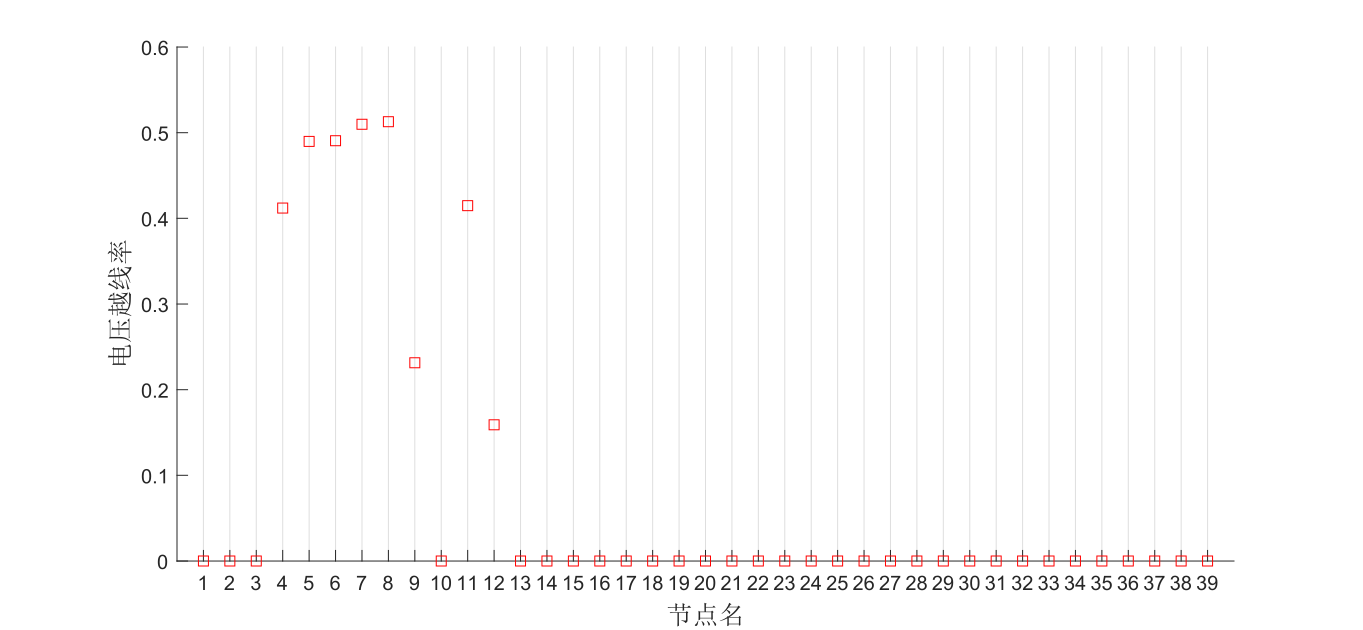
\includegraphics[height=7.9cm]{proCLiuLoad39.pdf}
  \caption{随机性风速、负荷下的概率潮流}
  \label{fig:proCLiuLoad39}
\end{figure}

\section{本章小结}
\label{sec:sum3}
本章节通过研究含风电电力系统自身存在脆弱性的原因,得出系统脆弱性的本质和系统脆弱性的数学描述,在此基础上,结合前人的研究,得到了含风电电力系统的脆弱性的定义。针对该定义,本文将系统的脆弱性分为结构脆弱性和状态脆弱性。

在系统的结构脆弱性定义的基础上,分别基于复杂网络和$PangRank$进行建模。针对各自的模型进行脆弱性研究,分别得出了电气度、电气介数和$PR$重要值的算法。前二者更关注的是支路上的潮流分布对拓扑的影响,而后者更在意的是有向的链接关系对拓扑的影响。本文以$IEEE14$系统为例,使用两种方法建模计算并进行了比较,认为二者分别从不同的角度对拓扑的脆弱性进行了研究,均具有实际意义。

在系统的状态脆弱性定义的基础上,首先分析了含风电电力系统的几种运行状态的意义。在此基础上,采用蒙特卡洛的方法将系统运行状态处于脆弱域时的不确定性进行量化,即使用概率统计的方法研究系统的状态脆弱性。以$IEEE39$系统为例,研究了在风速和负荷变化的情况下,系统各节点的状态脆弱性。本章通过研究系统的结构和状态的脆弱性,确定了脆弱性问题的具体研究内容,为之后建立含风电电力系统脆弱性量化评估模型奠定了理论基础。




